\documentclass[border=0mm]{standalone}

\usepackage{import}
\subimport{../../../}{preamble.tex}

\usepackage{tikz}
\usetikzlibrary{calc}
\usepackage{pgfplots}

\begin{document}

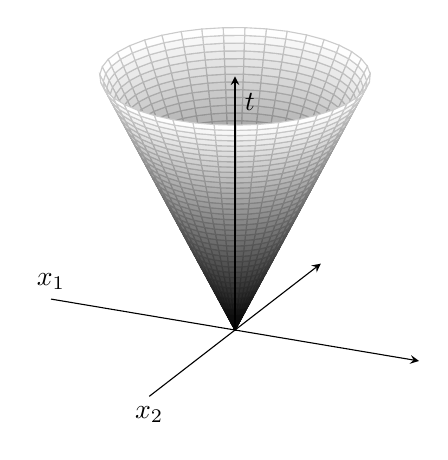
\begin{tikzpicture}
  \begin{axis}[
    axis lines=center,
    axis on top,
    xlabel={$x_1$}, ylabel={$x_2$}, zlabel={$t$},
    domain=0:1,
    y domain=0:2*pi,
    xmin=-1.5, xmax=1.5,
    ymin=-1.5, ymax=1.5, zmin=0.0,
    every axis x label/.style={at={(rel axis cs:0,0.5,0)},anchor=south},
    every axis y label/.style={at={(rel axis cs:0.5,0,0)},anchor=north},
    every axis z label/.style={at={(rel axis cs:0.5,0.5,0.9)},anchor=west},
    samples=40,
    z buffer=sort,
    colormap/blackwhite,
    ticks=none
    ]
    \addplot3 [surf] ({x*cos(deg(y))},{x*sin(deg(y))},{x});

  \end{axis}
\end{tikzpicture}

\end{document}

%%% Local Variables:
%%% mode: latex
%%% TeX-master: t
%%% End:
